% this TeX file provides an awesome example of how TeX will make super 
% awesome tables, at the cost of your of what happens when you try to make a
% table that is very complicated.
% Originally turned in for Dr. Nico's Security Class
\documentclass[11pt]{article}


% Use wide margins, but not quite so wide as fullpage.sty
\marginparwidth 0.5in 
\oddsidemargin 0.25in 
\evensidemargin 0.25in 
\marginparsep 0.25in
\topmargin 0.25in 
\textwidth 6in \textheight 8 in
% That's about enough definitions

% multirow allows you to combine rows in columns
\usepackage{multirow}
% tabularx allows manual tweaking of column width
\usepackage{tabularx}
% longtable does better format for tables that span pages
\usepackage{longtable}

\usepackage{graphicx} % allows inclusion of graphics

\usepackage{cite}


\begin{document}
% this is an alternate method of creating a title
%\hfill\vbox{\hbox{Gius, Mark}
%       \hbox{Cpe 456, Section 01}  
%       \hbox{Lab 1}    
%       \hbox{\today}}\par
%
%\bigskip
%\centerline{\Large\bf Lab 1: Security Audit}\par
%\bigskip
\author{Zander Mausolf}
\title{Assessment of TDKENO/MOOSE Coupling for Simulating Transients with Thermal Feedback}
\maketitle

\section{Introduction}
The accurate simulation of transient experiments typically requires thermal feedback to account for a variety of phenomenon such as Doppler broadening. To improve the transient analysis code TDKENO an investigation has begun into the best methods for incorporating thermal feedback. A large motivation is to improve the capabilities of modeling the TREAT reactor at the INL. TDKENO has proved capable of calculating values in agreement with TREAT experimental values.  The caveat is it has relied on feedback provided through empirical TREAT data, thus not making the approach robust.
The rapid transient conditions induced in TREAT experiments deposits significant heat quickly into the core and then rapidly cools.  Unlike commercial LWRs and BWRs there is no water moderator/coolant to complicate the heat-up model.  To better simulate these experiments it is desirable to utilize a simple heat-up model coupled to a neutronics solver. The primary objective is to be able to update the cross sections at the new temperatures to account for Doppler Broadening, which is thought to influence the TREAT experiments greatly.  

\section{Overview of TDKENO}

TDKENO is a transient analysis tool that solves the time dependent Boltzmann transport equation with the explicit representation of delayed neutrons. It does so with the Improved Quasi-Static (IQS) Method, which allows for the flux profile vary in time.  The main difference between the original Quasi-Static and IQS is the time derivative in IQS is handled explicitly with a backwards Euler approximation \cite{goluoglu2001time}. 

The basic assumption in IQS is that the total neutron flux can be factored into a shape and amplitude function \cite{Gehin}.  The amplitude function captures the time dependence and takes on physical significance by being cast into the form of the point kinetics equations as follows:

\begin{equation}
    \label{eq:pt_kin}
    \frac{dP(t)}{dt} = \frac{\rho(t)-\bar{\beta}(t)}{\Lambda(t)} P(t) + \sum_{j=1}^{6} \lambda_jC_j(t) + \bar{Q}(t)
\end{equation}

where $P(t)$ is the amplitude function, $\rho$ is reactivity, $\bar{\beta}$ is the effective delayed neutron fraction, $\Lambda$ is the generation time, $\lambda_j$ is the decay constant per neutron group $j$, $C_j$ is the density of delayed neutron precursors for group j, and $\bar{Q}$ is a source.

 Reactivity, generation time, etc. in TDKENO are found from their inner product definitions using a linearly interpolated flux shape. Exact expressions can be found in reference \cite{Bentley}.  Alternatively, these values may be computed during the Monte Carlo random walk but requires significant neutron histories to achieve low uncertainties \cite{Waddell}.  The shape function varies slowly in time and solves a modified version of the steady state transport equation.  The main modification here is an adjustment to the total cross section \cite{goluoglu2001time}\cite{Gehin}.  For this reason TDKENO calculations are limited to multi-group calculations, typically using 238 groups.  In TDKENO the shape equation is solved via Monte Carlo, but in principle the shape equation may be solved with deterministic methods.  Reference \cite{Shayesteh} provides an excellent rationale for implementing Monte Carlo techniques for the flux shape calculation.  A complete derivation of the IQS method used in TDKENO can be found in reference \cite{Bentley}. 
 
 The implementation in TDKENO is a hybrid in nature because it relies on a Monte Carlo calculation for the flux shape and a deterministic one for the point kinetics.  The Monte Carlo calculation coming from a modified version of KENO (either V.a or VI).  One can think of TDKENO as a solver of the point kinetics equations that drives the time dependence and calls upon KENO to provide the flux shape at desired times. 
 \begin{figure}
     \centering
     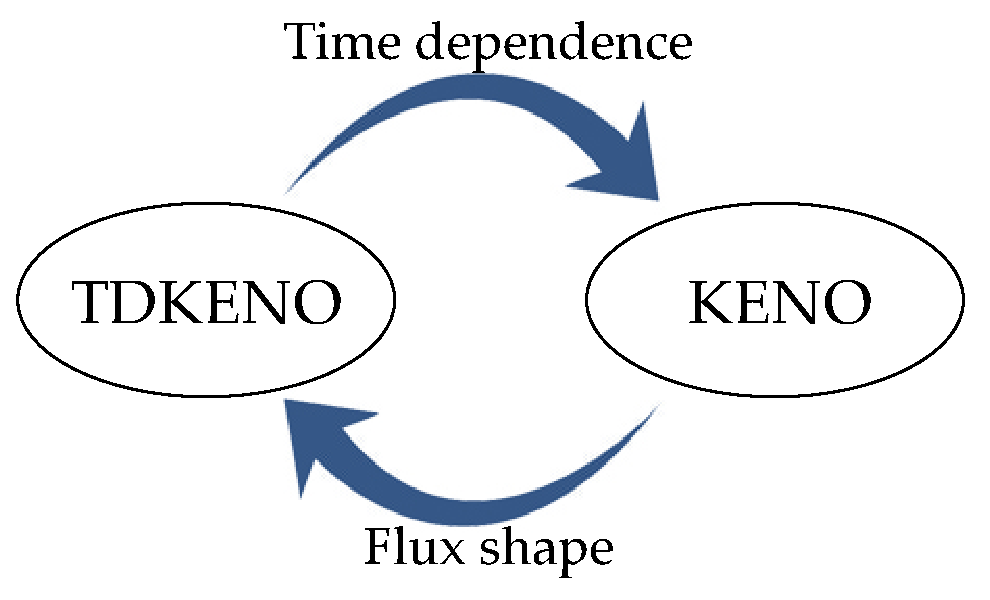
\includegraphics[width=8cm]{figures/tdkeno_flow.pdf}
     \caption{Simplified model of TDKENO calculation}
     \label{fig:simpletdk}
 \end{figure}

Applying this factorization to the three-dimensional time-dependent transport equation with the explicit representation of delayed neutrons results in a set of coupled equations.  Equations for the flux shape, amplitude, and delayed neutron precursors are solved on several time scales through an iterative process. The relative sizes are shown in Figure \ref{fig:time_scale}. 

\begin{figure}[h]
    \centering
    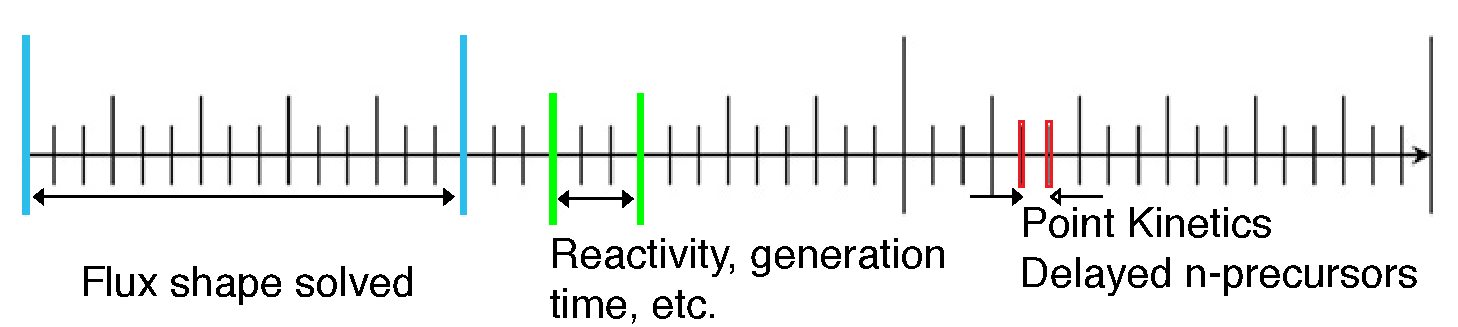
\includegraphics[width=10cm]{figures/time_scale.pdf}
    \caption{Time scale variation for IQS.}
    \label{fig:time_scale}
\end{figure}

The advantage of varying these time scales is less computational time compared to direct integration.  This comes from the flux shape being solved on a large time step. It is only done when the spatial distribution of neutrons changes significantly.  In between flux shapes, equation \ref{eq:pt_kin} is solved to capture the time dependent behavior.  Other IQS implementations are possible, such as the "Predictor Corrector" method.  Here one solves for the total flux and uses the shape in conjunction with the amplitude to correct the total flux \cite{Dulla}.  

 In its current formulation, TDKENO does not do this but rather lets the user define when a flux shape should be calculated.  This gives flexibility and may allow for computational savings as transients experience a rapid change in neutron distribution that is generally known about \emph{a posteriori} and rapidly come to a steady state. Therefore, a new calculation of the flux shape is not required.

\section{Current Status of TDKENO}
Feedback is incorporated into TDKENO specific to a problem.  For example an empirical model from historical data is implemented for TREAT specific problems. This model calculates a correction factor for the reactivity from the yield as follows:
\begin{equation}
    \rho_{fb}(t) = \sum_{i = 0}^{3}a_i Y^i (t)
\end{equation}
where $\rho_{fb}(t)$ is the feedback reactivity, $Y^i (t)$ is the total yield in the core at time $t$, and $a_i$ is the empirical coefficient for a third order polynomial.
  This provides reasonable answers but in previous simulations appears to differ significantly from experiment in calculating the peak power.  For the transient experiments simulated it over calculates the peak power significantly. However, the yield calculated agrees well with experiment.
Quenching coefficients and several problem specific feedback methods were included in the past.  A simple adiabatic model was put in place for a benchmark problem in \cite{Bentley}.  This is the closest to a generalized feedback model as was every attempted.  There is an obvious need for a more generalized feedback method and one that captures the physics better.  The IQS methodology complicates this with several time scales and complex iterative scheme.  

\section{Method for Incorporating Thermal Feedback}

For TREAT experiments and most transients, the thermal effect that needs to be resolved is the Doppler broadening of cross sections.  As the reactor increases in temperature the cross sections are broadened.  These changes in cross sections propagate through the entire problem.  Without feedback or with incorrect feedback the cross sections will not be updated and the results will differ from experiment.  Transients occur quickly and therefore can be looked at with models as simple as an adiabatic heat-up model.  From conversations with others working on TREAT the clipped transients work well with this model.  The next improvement, we believe for shaped transients, is to look at a steady state heat equation to capture the thermal conductivity effects.  The ultimate goal for reactors beyond TREAT is to couple the neutronics of TDKENO with a CFD (computational fluid dynamics) or TH (thermal-hydraulics) specific code.  Conventional reactors are moderated with water that may be in several phases.  Simple thermal models generally do not work with systems such as these.  As the goal is first to understand TREAT we looked at incorporating the adiabatic and a heat conduction model.

\subsection{Internal coupling}
 Two or more code bases may be built together such that one may call the others routines and pass data around in memory.  The most desirable option would be to build TDKENO under the MOOSE framework.  That would enable data to be based around instead of being written out and read by another program.  The difficulty in internally coupling TDKENO is the vastly different structures and less formal software development practices within TDKENO.  One such difficulty is TDKENO being written in Fortran 90.  Talking with Cody at the MOOSE team, Fortran 90 is slightly more difficult than other programming languages because of it inconsistent name mangling.  He said it is definitely possibly though, and they have built legacy programs within MOOSE before.  However, he said each time it was a unique problem and challenging.  Something that in itself may take the whole summer.  Looking to get some kind of results by the end of the summer I did not opt for the internal coupling method.

\subsection{External Coupling}
External coupling generally refers to code coupling methods build exclusively and rely on passing around input/output files to achieve coupling of data.  These methods are not as clean or robust but may be quicker to implement. This has an additional benefit in that KENO does not have to be built under the MOOSE framework, keeping TDKENO open to the possibility of using a different solver for the flux shape.  The reliance on KENO as the flux shape solver will be addressed in the future work section. 

\section{External Coupling Implementation}

The basic strategy of coupling MOOSE and TDKENO externally is to write out the necessary information with several scripts to parse data and call either program. This turned out to be the non-trivial to do in generality. 

The fundamental issue with coupling TDKENO/MOOSE is the different approach to modeling the geometry each takes.  TDKENO models the system utilizing KENO's Monte Carlo geometry, where shapes are defined by quadratic functions and referred to as CSG (combinatorial solid geometry). This allows for relatively simple definitions of the geometry to enable a system to be modeled almost exactly. MOOSE is a finite element analysis tool and requires a mesh to determine the geometry.  This is typically less detailed and more difficult to create than with Monte Carlo geometry implementations.  Looking through the literature and KENO manuals there was no clear method for mapping information between CSG and mesh based geometries.  Additionally, KENO has no generic interfaces for multi-physics coupling.  Several strategies were investigated to create a generic enough mapping of information between the two codes. 
The first was to tally the fission density on top of the Monte Carlo geometry.  This is already possible in KENO.  The user defines a Cartesian grid, specifying the height, width, depth and number of points in-between.   The fission density is then found in each section of this Cartesian geometry.  The discretization would have to be done such that the grid defined would match up to fuel elements.  If done this would provide the fission density in each fuel element.  If the CSG geometry defined fuel elements did not align with the grid then fissions may be tallied over larger or smaller regions than they should.  The result would some fuel elements appearing to have artificially larger or lower temperatures.  While not ideal in principle it is possible to define a grid that lines up well with the existing geometry.  

FIG. Of TREAT WITH KENO GEOM and mesh 

KENO writes out this tally style "mesh" in a proprietary file type with the extension .3dmap that may be read by several SCALE applications.  There are tools within SCALE to convert these file types to more generic ones such as VTK and SILO.  The VTK format, supported by VisIt, seemed the most appropriate as it appeared MOOSE could read those formats.  Upon further inspection was not entirely true. MOOSE is only able to read unstructured XML based VTK files.  This is a newer more robust format that is used by VisIt and supported by LibMesh.  So the simple convertor already available in SCALE was not useful as it was only able to convert from .3dMap to rectilinear VTK format.  In principle it would be possible to modify MOOSE to read these formats but would require significant changes according to the MOOSE team.  

The next thought was to convert from VTK rectilinear to VTK-XML unstructured.  It was possible to convert to XML with a GUI tool in VisIt but it remained a structured mesh.  With no way to map this KENO information into MOOSE the VTK XML was converted to .XYZ format.  This was read into moose and captured the nodal points correctly but all of the associated information about the fission density was lost. Directly converting the KENO mesh for MOOSE appears to require significant manipulation of both codes.
	One more approach was attempted. That was incorporating the Exodus II API to construct a mesh directly from the KENO data.  Exodus is the preferred format in MOOSE.  The API allows for creation of exodus meshes fairly simply.  The difficulty came in the format KENO stored everything made the mapping between nodal points confusing and difficult to come up with a scheme that would work in general.  
	
3dMap → VTK (rectilinear) → VTK XML → MOOSE? 

3dMap → VTK (rectilinear) → VTK XML → XYZ → MOOSE?

3dMap → VTK (rectilinear) → Exodus II→

3dMap → Exodus II → MOOSE

Instead of converting the mesh into a format the MOOSE can already read it seemed reasonable to construct a mesh in MOOSE and map values onto that mesh that approximately represents the geometry in KENO.  This seemed simpler as one can query mesh points in MOOSE and add values to it on the fly.  Instead of utilizing the .3dmap based mesh problem was discretized based on each fuel element of TREAT.  Note, this method is not robust and generally would only work for simple heat-up problems like in TREAT transients.  The fission density per unit was already given in KENO without additional tallies.  Our model of TREAT is organized into units of fuel elements positioned based on its location within a 2D array. See the figure below.  A unique unit may be constructed so the fission density is not averaged over similar units that are repeated.  Since the units were arranged into an array it is relatively simple to get create the geometry in 2D and capture the radial fission or flux distribution.  Furthermore additional discretization may not have been useful due to the method our model was created and how the cross sections are generated.  Each fuel element unit has several materials in it that are used to create multi-group cross sections. These materials may be re-used and therefor the cross section values re-used.  Even in different parts of the core at possibly different temperatures.  Updating the cross sections to new temperatures means assigning unique materials a new temperature and having that material correspond to a unique unit.  

\begin{figure}
    \centering
    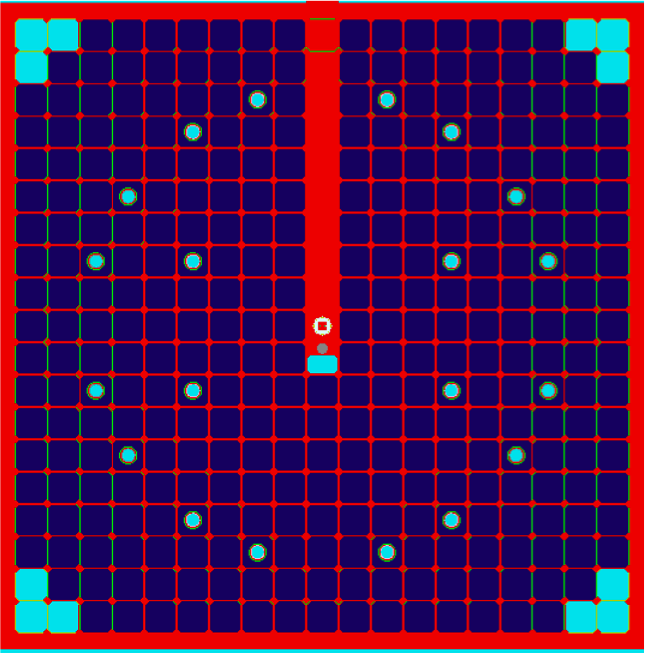
\includegraphics[width=10cm]{figures/treat_top_view.png}
    \caption{Overview of TREAT model in two dimensions}
    \label{fig:treat2d}
\end{figure}

A pseudo-mesh was created based on the location of each fuel element in 2D with the corresponding fission density, temperature.  A series of python scripts parse the KENO outputs to gather the fission density, create an (x,y) location for the center of each fuel element, and calculate the power density. It should be noted that KENO automatically provides the fission density in units of fissions/$cm^3$ and normalized per source neutron. The power density at first is calculated simply by multiplying the fission density by the average release per energy for U-235.  In reality this energy/fission value is more complicated to calculate but for an initial test the simpler option was chosen.  

	Next, we move on to working on the MOOSE side.  The goal is to solve the heat conduction problem with the heat source as the calculated power density. A heat conduction module is already available within MOOSE.  This was modified slightly to read in the text file produced from the KENO data and assign a different thermal conductivity value and power density at each quadrature point.  The mesh generated in MOOSE is created a priori to have approximately the same dimensions in 2D as the TREAT problem.  The KENO data was really providing values on nodal points but the values needed to be assigned on quadrature points, which are slightly offset from the nodal points.  This was achieved by simply determining the absolutely closest point from the KENO data to the corresponding quadrature point. 
	
\begin{figure}
    \centering
    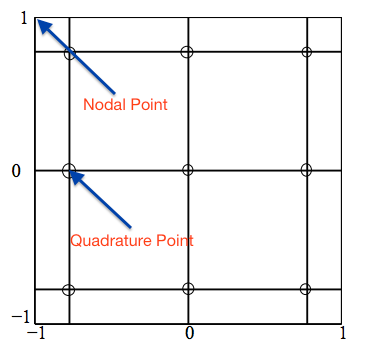
\includegraphics[width=10cm]{figures/nodalvsquad.png}
    \caption{Difference in nodal and quadrature mesh points}
    \label{fig:nodalquad}
\end{figure}

\section{Cross-Section Processing}
No matter the method of coupling, to capture the affect of Doppler broadening,  cross sections must be updated to the new temperature. Several approaches are possible:

1)	Updating the cross sections by creating a new set each time with the CENTRM/PMC utility. Because CENTRM/PMC calculates a problem-dependent flux profile, it provides a rigorous cross-section treatment that explicitly handles effects from overlapping resonances, fissile material in the fuel and surrounding moderator, anisotropic scattering, and inelastic level scattering \cite{bowman2007overview}.  Basically, once MOOSE has calculated a new temperature for each fuel element this information is mapped back to the KENO input file.  Each units mixture has a new temperature.  This input file is then processed with CENTRM/PMC to create unit dependent cross sections  based on the new temperature.  In most cases the unit will correspond to a unique fuel element. The cross section is then saved and placed in the TDKENO working directory.  The cross section creation time takes several minutes typically but does add another layer of complexity to the problem.  

2)  Instead of calculating the cross sections for each update of the temperature several cross sections for the same geometry may be made available before hand and interpolated within TDKENO to get as close to the new temperature as possible.  This requires knowing the range of temperatures the problem will be at.  For TREAT and many problems this is known.  The approach still is not as robust as the first likely not as accurate as it relies on interpolation.

Other coupled codes rely on code-specific features to handle the temperature distribution.  For instance Serpent allows the cross sections to be updated on the fly with the Target Motion Sampling (TMS) temperature treatment \cite{viitanen2012explicit}. Additionally, Serpent may model a continuously varying density distributions \cite{leppanen2013modeling}.  The variation of density may be important in future problems so it is important to keep in mind.  
OpenMC and MOOSE have been coupled as well.  The cross section updates are performed with an on-the-fly windowed multi-pole method for cross section Doppler broadening \cite{josey2016windowed}. This avoids interpolation of pre-generated cross sections or and weighting factors.  

Methods in OpenMC and Serpent are indeed very useful but may not be feasible options with the current reliance on KENO for the flux shape.  Each of these cross section processing methods relies on intricate processes that are ingrained in each respective code.  Mimicking such approaches would require significant modifications to KENO.  

The MC21 Monte Carlo code implemented a clever "source" and "sink" approach where the user dictates how the heat flows in the problem on top of the existing CSG geometry \cite{griesheimer2008integrated}.  This requires lot of user pre-processing but requires no meshes or discritizing the geometry beyond what is already defined.     



\section{Future Work}
All of the pieces are near  completion for a rudimentary coupling of TDKENO of MOOSE to capture  thermal affects.  Given the time constraints it was not possible to complete a robust method to couple TDKENO with MOOSE.  There are several different options that may be pursued in the future to develop a robust code to simulate transients with accurate thermal feedback. Several will be outlined below. 

\subsection{Build TDKENO as a MOOSE App Explicitly}  
A natural extension of the summer work would be to build TDKENO under the MOOSE framework.  This would require a robust 3D mapping strategy from CSG geometry to meshes MOOSE understands.  Presumably as MOOSE evolves it will become more robust and this may become easier.  Thus far it as proved challenging but it is out of the scope of possibilities.   
There are several advantages to this method
\begin{itemize}
    \item The internal coupling makes the coupling easier to adapt and improve. 
    \item As development progresses the solves on the MOOSE side may be made more complex to understand other phenomenon. For instance thermal expansion may be incorporated.  
    \item Utilize other applications and modules within MOOSE to understand new physics. 
\end{itemize}
There are significant disadvantages to this approach:

\begin{itemize}
    \item May have to build some SCALE based programs within MOOSE. Not a requirement but would make the coupling a bit "cleaner".  It is difficult as it is to build the latest version of SCALE (6.2) with the build system created at ORNL. Definitely would be a challenge in itself to migrate parts of SCALE over.
    Could opt to build the KENO/CENTRM executable separately and only call them when needed.  The “TDKENO” portion, basically the point kinetics solver/flux modifier would be built under MOOSE.
    \item Mapping from a CSG geometry to MOOSE type meshes is non-trivial.  A large point of using Monte Carlo is to get around the mesh creation portion of a simulation. Looking through the literature there are almost no coupled codes with KENO because of challenges like this.   
\end{itemize}

\subsection{Modify TDKENO to utilize a different Monte Carlo solver for the flux shape}
	In its current implementation TDKENO only calls upon a modified version of KENO to perform the flux shape.  The behaviour is akin to an externally coupled code, with "TDKENO" driving the time dependence and calling KENO when it needs the flux shape. Presumably other codes could accomplish the same task
	
	Modify TDKENO to not utilize KENO for the flux shape calculation.  Instead base it on a code such as Serpent or OpenMC with established multi-physics interfaces. 

a.	Some disadvantages.  These codes are not as mature, do not all possess the same features as KENO.  For instance in performing the adjoint calculation.   Require lots of rewriting of KENO possibly new formulation of the governing equations.

b.	Advantages.  Established multi-physics interfaces.  Lots of reference points and code already made for thermal feedback within MOOSE/each respective code. Modern codes may be easier to manage in the future. 

3)	To capture the temperature dependence the fission/power density may be tallied as a distribution based on Zernike polynomials.  Keep the coupling somewhat external.  The coupling would be simplified since only the Zernike

a.	Disadvantages.  Further reliance on KENO.  Modifying KENO source code can be challenging.  A newer methodology and it is not widely implemented.

b.	Advantages.  Construct almost exactly temperature distribution in great detail without discretizing the geometry from the CSG format.  Only have to pass around coefficients and read the temperatures from MOOSE.  Has been done in Serpent (in progress at INL), OpenMC but for Zernike polynomials that are orthogonal only circular domains.  

i.	It is possible to have Zerneki polynomials orthogonal on polygons (for radial dependence) with greater than 3 sides.  It has been show in some optics papers from 2015.  The example given provided a general methodology for P>3 sided polygons and a specific case of an 8 sided polygon with equal length sides.  For the TREAT problem the 8-sided case would need to be modified for sides that are not all the same but with two sides.  It seems in principle possible.  This would be a great solution for the TREAT problem. Could obviously be extended to cylindrical fuel elements with some ease.  It doesn’t make this methodology super robust as it relies on having fuel elements with a specific geometry.  For instance pebble bed reactors would be incompatible with this implementation. 

4)	Solving the heat conduction problem via Monte Carlo techniques.  There has been some work over the last 50 years on solving the heat conduction equation with a Monte Carlo approach.  Since the diffusion approximation in transport theory is mathematically equivalent to the heat conduction problem there are many analogous methods.  There is a fair amount of work published on this approach but nothing too mature.  Citing various computational difficulties and technical challenges. 

a.	Disadvantages.  Computational time may be larger than deterministic.  Require significant programming from the ground up.  May be tied to a specific geometry introduced by the neutronics solver.  No ties with MOOSE.

b.	Advantages.  Extremely robust!  Can solve problems with complex geometries with no discretization beyond the CSG description.  More novel research than existing coupling strategies?

\section{Conclusions}

\bibliographystyle{unsrt}
\bibliography{bibliography}

\end{document}

